The GMCF performance evaluation discussed in Section~\ref{sec:GMCFLESEval} was
the first ever to be conducted on the framework. The results discussed in the
evaluation were the final best results obtained after a number of changes were
made to the framework to improve performance.

Also, during development of the GMCF parallelised LES, an unusual bug was
encountered caused by Fortran and C++ interoperability through POSIX threads.
The bug is not framework specific but will be discussed in
Section~\ref{sec:fortrancppinteroperability} as it is applicable to any
application using POSIX threads to call Fortran subroutines.

\subsection{Performance improvements}

\begin{figure}
    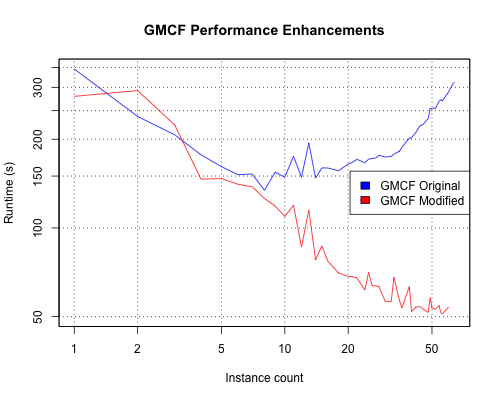
\includegraphics[width=0.5\textwidth]
    {graphs/GMCF-before-after-fixed-area.png}
    \caption{GMCF Before and After}
    \label{fig:gmcfbeforeandafter}
\end{figure}

\begin{table*}[t]
    \centering
    \begin{tabular}{|l|l|l|}
        \hline
        Change & 64 thread runtime (seconds) & Performance Improvement\\
        \hline
        Original & 320.8 & -\\
        \hline
        Global reduction changes & 150.8 & 53\%\\
        \hline
        Spin lock and busy waiting on FIFOs & 120.6 & 20\%\\
        \hline
        Thread Pinning & 100.1 & 17\%\\
        \hline
        Map of FIFOs & 80.1 & 20\%\\
        \hline
        Not sending REQDATA packets & 56.1 & 30\%\\
        \hline
    \end{tabular}
    \caption{Summary of performance enhancements made to GMCF}
    \label{tab:gmcfperformanceimprovements}
\end{table*}

\begin{table*}[t]
    \centering
    \begin{tabular}{|l|l|l|}
        \hline
        Global reduction method &
        4 thread message rate per second &
        64 thread message rate per second\\
        \hline
        Original GMCF & 9,842 & 60\\
        \hline
        PThread Mutex and condition variables & 29,960 & 120\\
        \hline
        PThread Spin locks and busy waiting & 1,371,846 & 5,234\\
        \hline
        MPI All\_Reduce & 1,344,086 & 53,504\\
        \hline
    \end{tabular}
    \caption{Global Reduction microbenchmark results}
    \label{tab:gmcfglobalreductionresults}
\end{table*}

Figure~\ref{fig:gmcfbeforeandafter} shows the original GMCF performance results
alongside the best results for a fixed area run. As is clear from the graph,
GMCF was suffering from scalability issues, with the runtime increasing above
ten threads and causing a bathtub curve. As
Table~\ref{tab:gmcfperformanceimprovements} shows, a number of framework changes
including a dedicated method of calculating global reductions, spin locks, and
thread pinning were investigated and were ultimately implemented to improve
performance. Overall these changes were responsible for making GMCF performance
scalable as the number of threads grows and reducing GMCF performance to nearly
one sixth for a fixed area problem.

\subsubsection{Global Reduction}

The first task in the performance investigation was to look for aspects of
communication that were causing the bathtub curve. The performance degradation
at ever increasing levels of threads pointed towards global communication. Only
one kind of global communication occurs in each LES time step, global
reductions. The maximum, minimum, and sum of a small number of scalars is
required. One of those reductions, a global sum, is contained within an inner
loop and is thus calculated up to fifty times per main loop iteration.
Temporarily disabling this global sum caused the runtime graph to flatten out
without significant runtime degradation at higher threading levels. Runtime was
now around 150 seconds rather than nearly 320 seconds at 64 threads which was a
significant improvement but still nearly six times slower than MPI.

With the cause of the bathtub curve found, a number of different ways of
calculating a global reduction were investigated. A summary of microbenchmark
results for the different methods tried is shown in
Table~\ref{tab:gmcfglobalreductionresults}. The original method involved message
passing in the same way halo exchanges and other arrays were passed. The
overhead of sending packets for a single scalar were clearly significant. Also,
a single thread was the recipient of all of the scalars, one from each thread.
That same thread then calculated the global reduction, then sent the result to
every other threads. This caused a single thread to have an ever increasing
amount of work to do compared to other threads, a problem that became worse as
the total thread count grew. In a micro benchmark, GMCF was over 100x slower
than MPI when calculating a global sum over 4 threads and nearly 1000x slower
over 64 threads.

The solution was a specific subroutine embedded within the GMCF framework that
did not use messages but instead a global variable. Rather than have a single
thread do the heavy lifting of receiving, calculating, and sending results, each
thread accessed the global variable and did a partial calculation. Once all
threads had done the partial calculation, all threads can then simultaneously
read the global variable to get the final result. Two methods of this were
investigated with the first using mutexes and condition variables to mediate
access to the global variable. The mutexes and condition variables method
improved performance by 2-3x over the GMCF message passing implementation but is
still significantly slower than MPI. The final implementation involves a POSIX
thread spinlock and busy waiting. This combination of spinlock and busy waiting
offered around a 45x improvement over the more traditional mutex and condition
variable combination. This brought performance for four threads inline with MPI
but performance for 64 threads is still an order of magnitude slower than MPI.

When the global reductions in LES were re-enabled to use the new method of
calculation, the global reduction overhead became negligible. This shows that,
although MPI's method of global reduction has better performance at higher
thread counts, the LES doesn't execute the global reduction often enough for
this to impact the overall runtime.

OpenMPI's method of global reduction uses a ``recursive doubling algorithm''.
This involves a tree-like reduction that in a work depth that is logarithmic
with the number of communicating processes. GMCFs new method has a work depth
that is linear with the number of threads

\subsubsection{Spin locks and busy waiting}

Traditional locks used for mutual exclusion will cause a thread to sleep if the
lock is held by another thread. Condition variables are also used to allow a
thread that currently holds the lock, but finds the data it has access to isn't
ready, for example a queue that is empty in a subroutine that processes the head
of a queue. These also cause a thread to sleep until a condition is met. In this
example, until the queue isn't empty. This stops a thread wasting CPU cycles and
is seen as a way to mediate fair access to a shared resource.

Spin locks replace traditional locks. If another thread holds the lock, rather
than going to sleep, a thread will ``spin'' over the lock, continually trying to
obtain the lock until the lock is available. Spin locks use atomic operations
such as compare and swap to implement this. This is thought to improve
performance in some cases. Anderson et al. \cite{Anderson1990} found that spin
locks offer poor performance, especially at high thread counts whereas
Mellor-Crummey et al. \cite{Mellor-Crummey1991} found that the lack of fairness
in spin locks can result in improved performance, likely due to the reduced
latency between a lock becoming available and another thread locking it.

Busy waiting replaces condition variables. Rather than sleeping until a specific
condition is met, a thread will enter an empty loop and continually check the
while condition. When the while condition is false, the thread knows it is safe
to execute the required action.

With the success of spin locks and busy waiting in the global reduction code
GMCFs per-thread receiving FIFO queues were looked at as another potential
source of performance improvement. Model threads will regularly sleep, waiting
for packets to arrive. This reduces CPU usage but increases the latency between
a packet arriving and a thread being awake and able to process it. MPI processes
do not sleep by default for this reason. The FIFO queues in GMCF were currently
managed by mutual exclusion locks and condition variables. These were replaced
with spin locks and busy waiting. This reduced runtimes by around 20\%, a
significant improvement.

This change is the reason behind the lack of 63 and 64 thread runs in the GMCF
evaluation. This is due to two non-model threads that are created by the GMCF
framework. These two threads currently use the same code for their FIFO queues.
As a result these two threads needlessly spin and waste the computational
resources of two cores. This is a temporary implementation detail as future work
will include creating a separate FIFO queue implementation for these threads to
allow them to sleep again.

\subsubsection{Thread Pinning}

POSIX threads, by default, are free to be mapped to any available CPU core by
the kernel. This can help kernels to even load over all of the CPUs but is not
ideal from a cache perspective. Each time a thread migrates to a different CPU
socket, the cache built up on that socket's cache is wasted. This can have a
significantly negative impact on performance.

To help combat this, GMCF threads were allocated a single core each. This is
identical to the behaviour of MPI's by-core mapping which helped to improve
performance for the MPI version of the LES. The thread pinning change in GMCF is
responsible for the slight degradation in performance at small numbers of
threads as shown in Figure~\ref{fig:gmcfbeforeandafter} but improved performance
at higher numbers of threads by around 17\%. Again, since the assumption is that
model simulations are the only running programs on a machine and thus use all
CPU cores available, this is a worthwhile change.

\subsubsection{Miscellaneous Changes}

In addition to lower level changes, framework-specific changes were also made.
For example, the original GMCF had one queue for each thread for each type of
packet. Since a thread may be looking for a packet from a specific thread, the
queues had to be iterated over to find a packet from the requested source
thread. To prevent this, each thread had a map of queues for each packet type
and each source thread. This meant that, to find a specific packet, only one
queue had to be looked at and the required packet is guaranteed to either be at
the head of the queue. This map of FIFOs helped speed up the code that waited
for and found packets resulting in an overall performance improvement of nearly
20\%.

Another change was to remove the need to send ``REQDATA'' packets. This packet
type is required for model coupling where a model can request data from another
model. This is necessary for model coupling since the two communicating models
do not know about each other explicitly. For model parallelisation this packet
type is unnecessary. Each thread for a model is able to work out which thread it
needs data from, and what data it needs to send data to. By removing the
unnecessary ``REQDATA'' packets from the GMCF LES, the number of packets sent
between threads was reduced by one third and runtime was reduced by around 30\%.

\subsection{Fortran and C++ interoperability issue}
\label{sec:fortrancppinteroperability}

The GMCF framework is written in C++ with a Fortran API. Since the LES is
written in Fortran, GMCF creates a number of POSIX threads, each of which calls
LES's main subroutine. All of the arrays the LES uses are allocated on the stack
thus making it seemingly trivial to show that each thread has an independent
copy of each variable.

Due to an implementation detail on Fortran stack variables, this is not the
case. Since Fortran has no built-in concept of a thread, the compiler is free to
change many aspects of the code that a compiler for a thread-aware language
could not do. One of these changes involves changing how large stack variables
are stored. Having large stack variables may not be performance optimal so the
Fortran compiler looks for large stack variables (32kiB or larger by default)
and allocates memory in ``static memory'' for them. The stack variable is then
silently replaced by a pointer to this area of memory.

For a single threaded application this change has no consequences as the thread
can still read and write to the array as normal. The problem occurs in a
situation such as in GMCF where multiple threads are calling the same Fortran
subroutine simultaneously. Rather than each thread having its own array on the
stack, they now all share a pointer to the same area in static memory. As a
direct result, any writes are visible to all threads resulting in erroneous
behaviour. From a developer's perspective, the behaviour is very confusing since
the code has an array on the stack, yet one thread changing its stack variable
seems to affect the other threads' stack variable.

The solution to this problem is simple. Rather than the arrays being coded as
being on the stack, the arrays are made allocatable and each thread, at runtime,
will allocate its own array on the heap. This can be automated since static
variables have their size known at compile time so a simple script can easily
work out and insert the required allocate calls. This stops the compiler causing
erroneous behaviour while only involving a minor code change with insignificant
runtime overhead for the allocation and deallocation.

\subsection{False Cache Sharing}

False cache sharing is where a single cache line contains some data only
accessed by one thread (called A) and some data only accessed by another thread
(called B). If thread A updates its data, thread B has to invalidate its cache
line even if the data it has access to hasn't changed. This can occur in
communication exchanges. The first part of a cache line may contain the last few
elements of an array that will be updated by thread A's bottom neighbour. The
latter part of a cache line may contain the first few elements of an array that
will be updated by thread B's top neighbour. Rather than one cache line
invalidation between threads, they will now experience two. This has obvious
performance issues but isn't easily resolved, if at all. Preventing false cache
sharing involves ensuring arrays are aligned in a cache line and no single cache
line contains data for multiple threads. This is impossible in the general case
as the fix involves padding an array to the size of a cache line. MPI cannot
suffer from this problem as MPI works on processes that, by definition, have
independent memory spaces.

To investigate this problem, a 4kB array was added to the LES model code. This
meant each thread had a 4kB padding between each threads. Performance was
investigated for both the fixed area and expanding area runs but the padding had
no effect on performance.

To further investigate the potential cache sharing option, a sleep based on a
thread's model ID was added. In addition to the padding array, the sleep forced
thread number i complete all of its allocate calls before thread number i+1.
This would give the best chance of removing the possibility that false cache
sharing would occur. Performance was investigated again but the padding and
sleep had no effect on performance.

This shows that there is no benefit from trying to pad the arrays since this
will not improve performance.
